\documentclass[aspectratio=169,11pt]{beamer}
\usepackage[utf8]{inputenc}
\usepackage[T1]{fontenc}
\usepackage{lmodern,amsmath,amssymb,booktabs,graphicx,listings}
\definecolor{ink}{HTML}{173342}
\definecolor{teal}{HTML}{127D92}
\definecolor{rust}{HTML}{C66C32}
\setbeamercolor{normal text}{fg=ink,bg=white}
\setbeamercolor{structure}{fg=teal}
\setbeamercolor{frametitle}{fg=ink}
\setbeamertemplate{navigation symbols}{}
\setbeamertemplate{footline}{\hfill\scriptsize Acemoglu \& Restrepo\quad\insertframenumber/\inserttotalframenumber\hspace{5mm}\vspace{3mm}}
\setbeamersize{text margin left=9mm,text margin right=9mm}
\setbeamerfont{frametitle}{size=\Large,series=\bfseries}
\setbeamerfont{title}{size=\LARGE,series=\bfseries}
\setlength{\parskip}{5pt}
\newcommand{\src}[1]{\vfill{\scriptsize\color{gray}NBER 22252, June 2017, #1.}}
\newcommand{\sh}{\widehat\sigma}
\lstset{basicstyle=\ttfamily\footnotesize,columns=fullflexible,breaklines=true,showstringspaces=false,literate={σ}{{$\sigma$}}1 {ε}{{$\varepsilon$}}1 {ℝ}{{$\mathbb R$}}1 {≠}{{$\ne$}}1 {∧}{{$\land$}}1 {←}{{$\leftarrow$}}1 {·}{{$\cdot$}}1}
\title{The Race between Man and Machine}
\subtitle{Tasks, wages, and the limits of formal verification}
\author{davidolano03}
\institute{Acemoglu \& Restrepo (2018), American Economic Review\\[5pt]
\href{https://github.com/davidolano03/ai-06-restrepo}{\texttt{github.com/davidolano03/ai-06-restrepo}}}
\date{AI and Economic Modeling\quad September 2026}
\begin{document}
\begin{frame}\titlepage
\vspace{-5mm}\centering\footnotesize Source read: NBER revision of June 2017, 87 pages\\
Working-paper title: \emph{The Race Between Machine and Man}
\end{frame}

\begin{frame}{The economic question}
When machines can perform more tasks, what happens to \textbf{wages, employment, and labor's share}?
\par\medskip
\begin{itemize}
\item Automation makes existing tasks feasible with capital.
\item New tasks give labor a new productive role.
\item Factor prices influence which tasks are adopted and which innovations pay.
\end{itemize}
\par\medskip
The unit of analysis is an \textbf{aggregate economy}. A worker's wage and the economy's labor share need not move together.
\src{pp. 1--6}
\end{frame}

\begin{frame}{Tasks and the adoption threshold}
\[
i\in[N-1,N],\qquad \gamma'(i)>0,\qquad I\in[N-1,N].
\]
Capital is technologically feasible only for $i\le I$. Firms compare unit factor costs:
\[
R\quad\text{versus}\quad\frac{W}{\gamma(i)},\qquad
\frac W R=\gamma(\widetilde I),\qquad I^*=\min\{I,\widetilde I\}.
\]
\begin{itemize}
\item Capital performs the lower tasks; labor performs the higher tasks.
\item Raising $N$ replaces the lowest task with a more productive one.
\item Task measure stays at one: new tasks change composition and quality.
\end{itemize}
\src{eqs. (1)--(6), pp. 6--8}
\end{frame}

\begin{frame}{The household and firms}
\[
\max_{C,L}\frac{(Ce^{-\nu(L)})^{1-\theta}-1}{1-\theta},
\qquad C=RK+WL,\qquad \nu'(L)=\frac WC.
\]
At $\theta=1$, utility is $\ln C-\nu(L)$. Capital is fixed in the static model.
\par\medskip
Competitive firms minimize each task's cost and the final producer combines tasks through a CES aggregator. Factor markets clear.
\[
L=L^s(\omega),\qquad \omega=\frac{W}{RK},\qquad
s_L=\frac{WL}{RK+WL}=\frac{\omega L}{1+\omega L}.
\]
Employment responds to the wage relative to capital income, not to the wage alone.
\src{eqs. (4), (8)--(11), pp. 7--10}
\end{frame}

\begin{frame}{Conditions behind the static results}
\begin{enumerate}
\item Positive, strictly increasing $\gamma(i)$: labor has comparative advantage in higher tasks.
\item $\eta\to0$ or $\zeta=1$: homothetic factor demand, with $\sh=\sigma(1-\eta)+\zeta\eta>0$.
\item Capital small enough that $R>W/\gamma(N)$: new tasks are used immediately.
\end{enumerate}
\par\medskip
Also: competitive production; the household's regularity and concavity conditions; positive labor-supply elasticity $\varepsilon_L$.
\par\medskip
For strict automation effects we need $N-1<I^*=I<\widetilde I$. At $I=\widetilde I$, left and right derivatives may differ.
\src{Assumptions 1--3; Propositions 1--3; footnote 15}
\end{frame}

\begin{frame}{Displacement and reinstatement}
\[
G=\int_{I^*}^{N}\gamma(i)^{\sh-1}\,di,\qquad a=I^*-N+1,
\]
\[
\Lambda_I=\frac{\gamma(I^*)^{\sh-1}}G+\frac1a>0,
\qquad\Lambda_N=\frac{\gamma(N)^{\sh-1}}G+\frac1a>0.
\]
With $K$ fixed and $I^*=I<\widetilde I$:
\[
\frac{d\ln\omega}{dI}=-\frac{\Lambda_I}{\sh+\varepsilon_L}<0,
\qquad\frac{d\ln\omega}{dN}=\frac{\Lambda_N}{\sh+\varepsilon_L}>0.
\]
Labor share and employment move with $\omega$. Automation displaces labor; new tasks reinstate labor demand.
\src{Proposition 2, pp. 11--12}
\end{frame}

\begin{frame}{The wage condition}
For a marginal increase in $I$, holding $N,K$ fixed:
\[
\underbrace{\frac{d\ln W}{dI}}_{\text{equilibrium wage}}
=\underbrace{\left.\frac{\partial\ln Y}{\partial I}\right|_{K,L}}_{g_I:\ \text{productivity}}
-\underbrace{(1-s_L)\frac{\Lambda_I}{\sh+\varepsilon_L}}_{D_I:\ \text{displacement}}.
\]
\bigskip
\centering\Large\color{teal}The wage rises if and only if $g_I>D_I$.
\par\par\medskip\normalsize\color{ink}\raggedright
Both effects are positive in magnitude. Labor share can fall while the wage rises. Productivity holds both factors fixed; the wage response allows employment to adjust.
\src{Proposition 3, pp. 12--14}
\end{frame}

\begin{frame}{A reproducible static experiment}
\[
\eta\to0,\quad\sigma=0.8,\quad \gamma(i)=e^{5i},\quad
B=1,\quad N=1,\quad I=0.4.
\]
Choose $\nu(L)=L^2/2$ and logarithmic utility. Then
\[
L^2=s_L,\qquad\omega=\frac{L}{1-L^2},\qquad
\varepsilon_L=\frac{1-L^2}{1+L^2}.
\]
\begin{itemize}
\item Solve employment and the adopted cutoff for 220 values of $K$.
\item Verify market clearing, household optimality and cutoff consistency.
\item Compare the analytical wage response with central differences.
\end{itemize}
\small Illustrative parameters, not empirical estimates. All retained points satisfy the new-task adoption condition.
\end{frame}

\begin{frame}{Productivity can dominate displacement}
\centering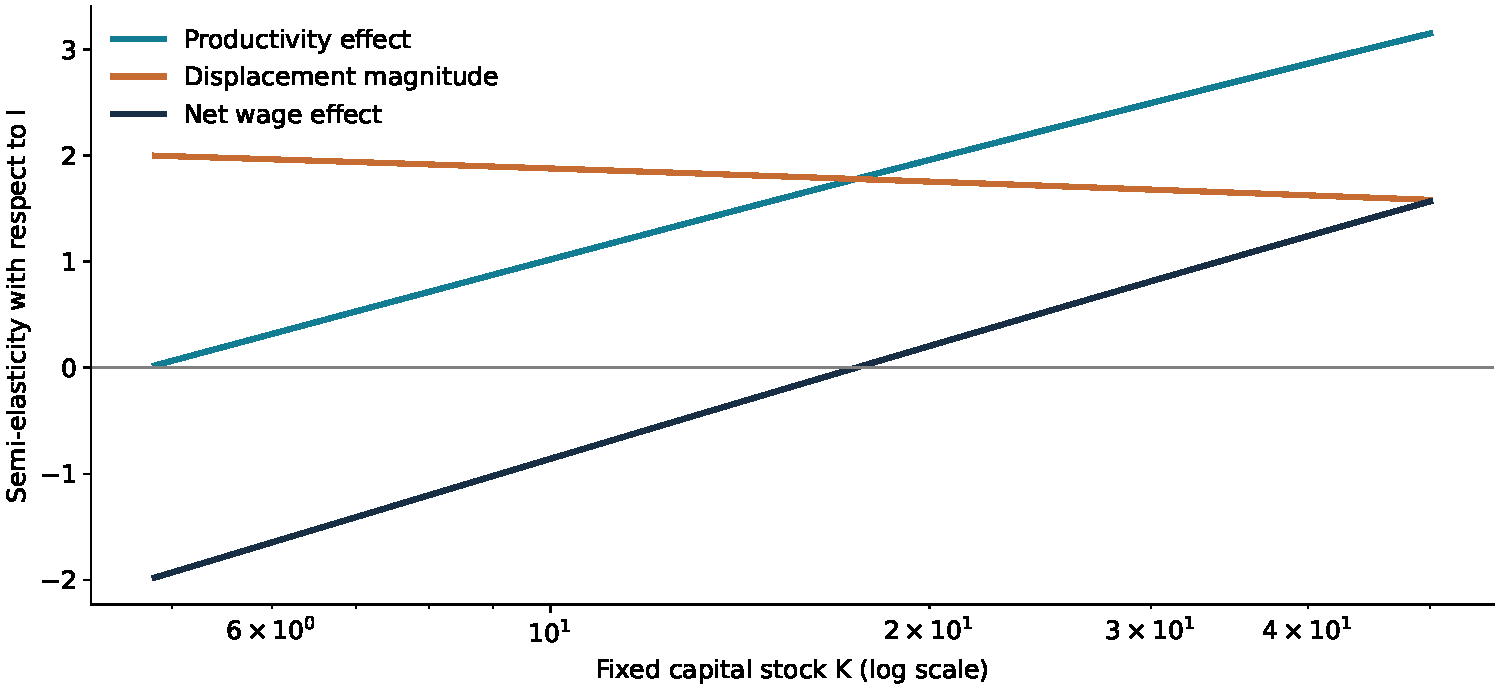
\includegraphics[width=.94\textwidth,height=.72\textheight,keepaspectratio]{figures/wage_decomposition.pdf}
\par\small Own computation; technology-constrained points only. Each derivative holds its displayed $K$ fixed.
\end{frame}

\begin{frame}{Two admissible wage responses}
\centering
\begin{tabular}{lrr}\toprule
 & Wage falls & Wage rises\\\midrule
Fixed capital $K$ & 8.370 & 32.834\\
Productivity $g_I$ & 0.777 & 2.612\\
Displacement $D_I$ & 1.909 & 1.663\\
$d\ln W/dI$ & $-1.132$ & $+0.950$\\
$ds_L/dI$ & $-1.375$ & $-1.299$\\
$dL/dI$ & $-0.916$ & $-0.811$\\\bottomrule
\end{tabular}
\par\medskip\raggedright
These are derivatives per unit of $I$, not percentage changes for a one-unit shock. Both cases satisfy $I^*=I<\widetilde I$ and $R>W/\gamma(N)$.
\small Maximum analytical/numerical wage-derivative error: $2.3\times10^{-9}$.
\end{frame}

\begin{frame}{Technological feasibility is not adoption}
\centering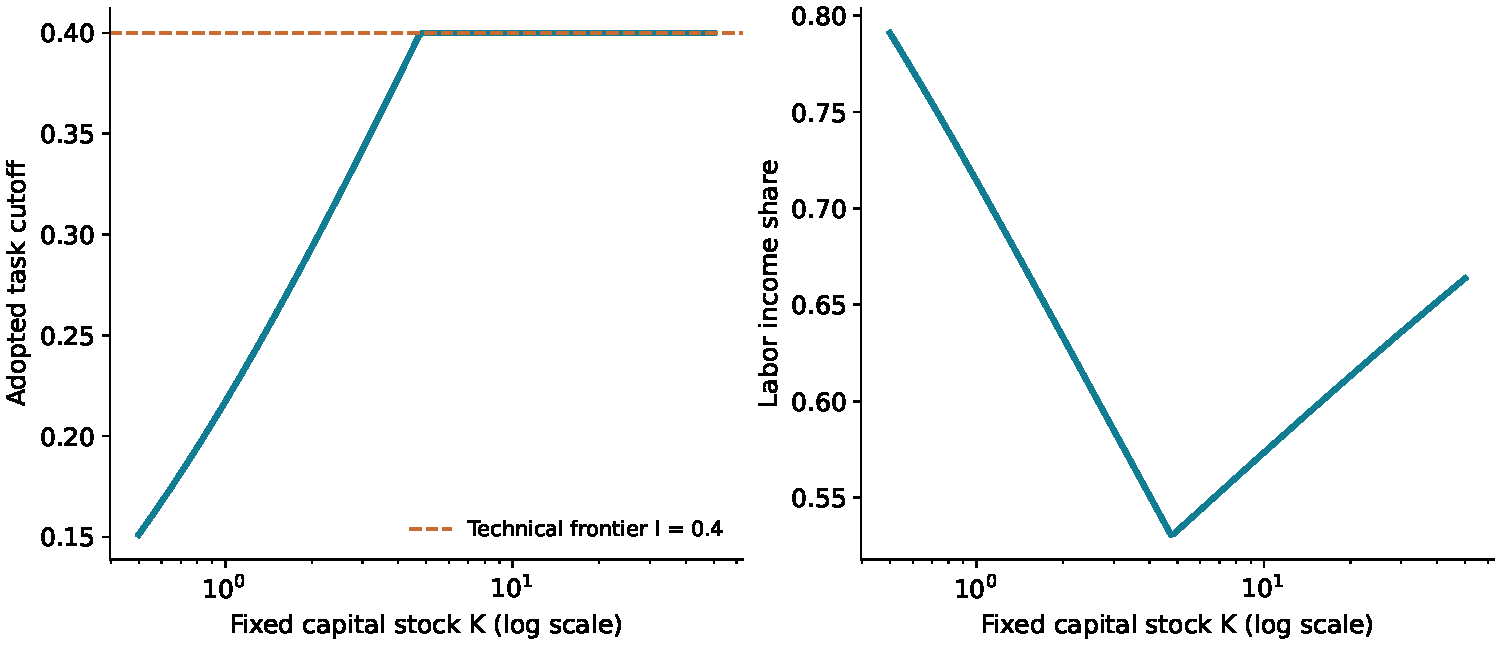
\includegraphics[width=.94\textwidth,height=.69\textheight,keepaspectratio]{figures/adoption_share.pdf}
\par\small At $K=0.5$, $I^*\approx0.151<I=0.4$. A small increase in $I$ has zero local effect. Cross-$K$ slopes are not automation effects.
\end{frame}

\begin{frame}{Balanced growth: a conditional result}
Proposition 6 assumes $\gamma(i)=e^{Ai}$, $A>0$, Assumption 2, $\sh>\zeta$, and sufficiently few scientists: $S<\bar S$.
\[
\rho>\bar\rho,\qquad\frac{\kappa_I}{\kappa_N}>\bar\kappa
\quad\Longrightarrow\quad
n=N-I\in(\bar n(\rho),1),\quad\kappa_Iv_I(n)=\kappa_Nv_N(n).
\]
\begin{itemize}
\item A unique interior balanced growth path balances the two innovations.
\item $\theta=0$: global saddle-path stability. $\theta>0$: local uniqueness and asymptotic saddle-path stability.
\item $\rho<\bar\rho$: a full-automation BGP exists. Other innovation-productivity ranges allow multiple BGPs or no automation.
\end{itemize}
\small Restoring forces after a temporary shock do not undo a permanent change in innovation incentives. Strict threshold equalities are not covered here.
\src{Proposition 6 and Corollary 2, pp. 25--28}
\end{frame}

\begin{frame}[fragile]{Mathematics, Lean translation, checked proof}
\small Reduced response equations ($w,r,\ell$ are candidate log changes):
\[
\sigma(w-r)+\ell=z,\quad\ell=\varepsilon(w-r),\quad sw+(1-s)r=g
\ \Rightarrow\ w=g+(1-s)\frac z{\sigma+\varepsilon}.
\]
\begin{lstlisting}
theorem solve_linearized_system
    (s sigma eps g z w r ell : Real) (hden : Not (sigma + eps = 0))
    (hdemand : sigma * (w - r) + ell = z)
    (hsupply : ell = eps * (w - r))
    (haccount : s * w + (1 - s) * r = g) :
    And (w = g + (1 - s) * (z / (sigma + eps)))
      (And (r = g - s * (z / (sigma + eps)))
        (ell = eps * (z / (sigma + eps)))) := by
  have hrel : w - r = z / (sigma + eps) := by
    apply (eq_div_iff hden).2
    nlinarith [hdemand, hsupply]
\end{lstlisting}
\scriptsize \texttt{MainTheorems.lean}, with ASCII variable names and \texttt{And}/\texttt{Not} notation. Opening proof fragment; full theorem compiles.
\end{frame}

\begin{frame}{What Lean verifies}
\begin{itemize}
\item $\mathbb R$ fixes the domain. The equations are explicit premises; $\sigma+\varepsilon\ne0$ makes division valid.
\item \texttt{eq\_div\_iff} converts a quotient identity to multiplication. \texttt{nlinarith} proves the polynomial consequence.
\item Setting $z=-\Lambda_I$ recovers the displacement decomposition. Two more contracts construct a reduced-system solution and positive productivity with a negative wage response.
\end{itemize}
\par\medskip
\textbf{Boundary:} these are three algebraic support contracts. Lean does not yet derive the response equations from the continuum economy, prove differentiability, or prove the paper's BGP results.
\par\medskip
\small Lean 4.30.0-rc2: focused proof build \textbf{exit 0}; required \texttt{--fast} check \textbf{exit 0}. Full semantic audit and source theorem coverage remain open.
\end{frame}

\begin{frame}{Hand check: employment and labor share}
\begin{columns}[T]
\column{.55\textwidth}
\centering
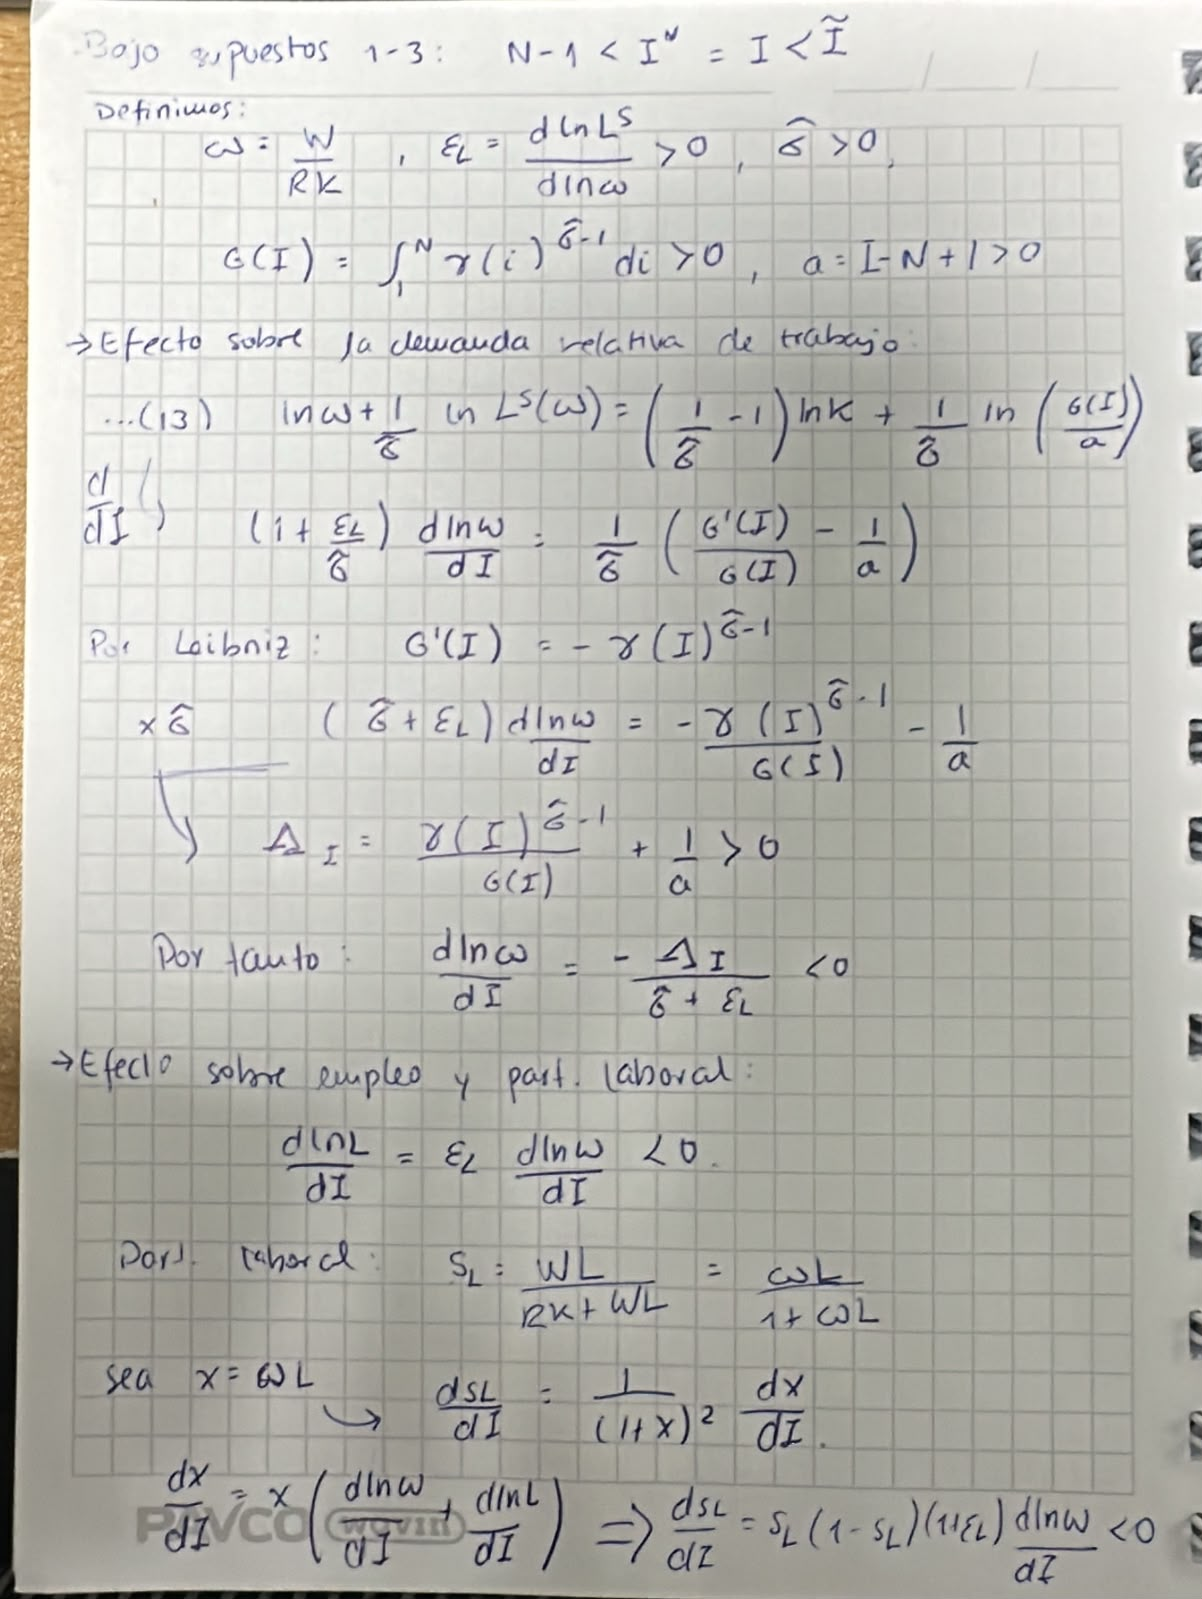
\includegraphics[width=\linewidth,height=.74\textheight,keepaspectratio,trim=0 0 0 650,clip]{hand/derivacion-01.jpg}
\par\scriptsize Detail from the student's first handwritten page.
\column{.42\textwidth}
\small With $K,N$ fixed and $I^*=I<\widetilde I$:
\[
\frac{d\ln\omega}{dI}=-\frac{\Lambda_I}{\sh+\varepsilon_L}<0.
\]
\[
\frac{d\ln L}{dI}=\varepsilon_L\frac{d\ln\omega}{dI}<0.
\]
\[
\frac{ds_L}{dI}=s_L(1-s_L)(1+\varepsilon_L)
\frac{d\ln\omega}{dI}<0.
\]
\textbf{Verdict:} displacement lowers employment and labor's share under the stated conditions. This does not determine the wage sign.
\end{columns}
\end{frame}

\begin{frame}{Hand check: the wage claim}
\begin{columns}[T]
\column{.55\textwidth}
\centering
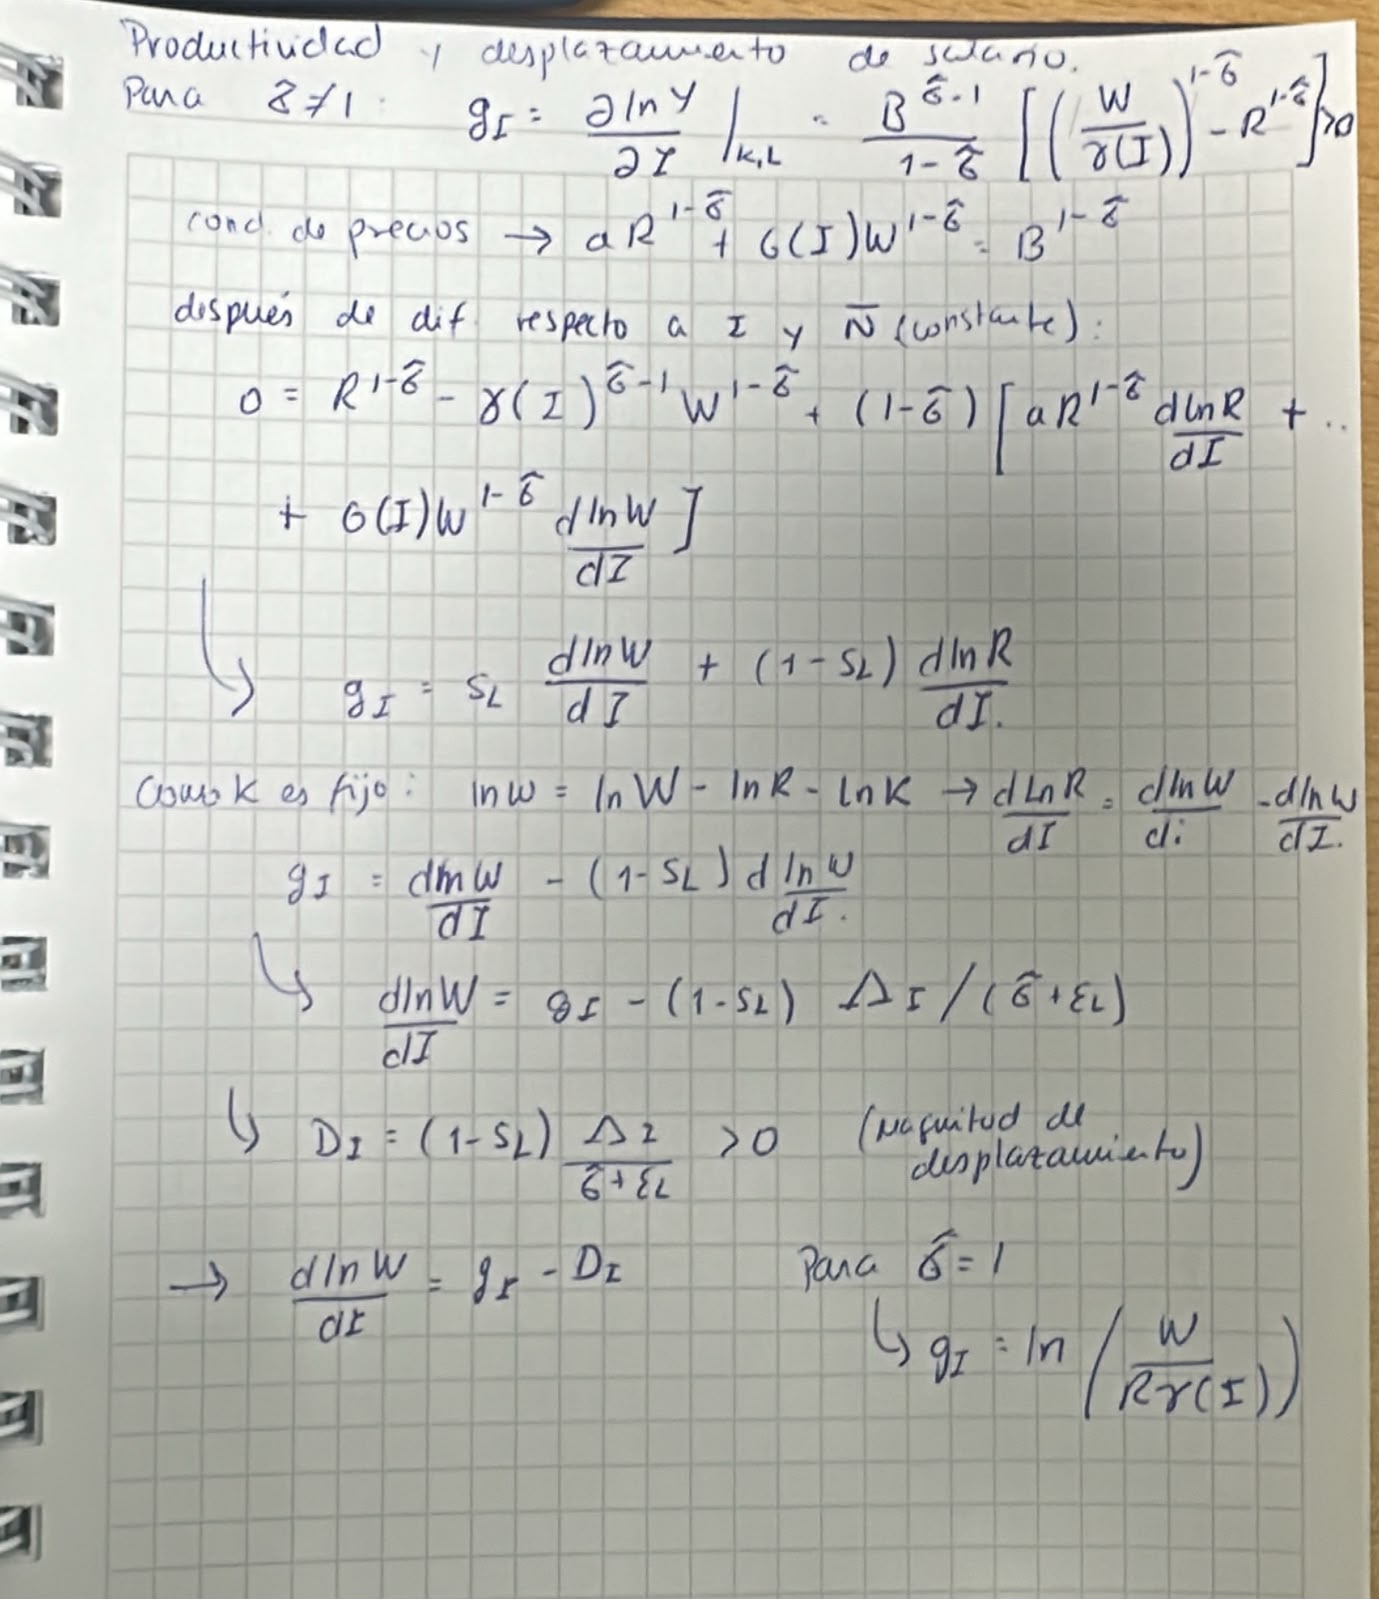
\includegraphics[width=\linewidth,height=.70\textheight,keepaspectratio,trim=0 0 0 820,clip]{hand/derivacion-02.jpg}
\par\scriptsize Detail from the student's second handwritten page.
\column{.42\textwidth}
\small \textbf{Claim to test:} ``Automation necessarily lowers wages.''
\[
\frac{d\ln W}{dI}=g_I-D_I,
\]
\[
D_I=(1-s_L)\frac{\Lambda_I}{\sh+\varepsilon_L}>0.
\]
\textbf{Verdict:} false in general. The wage rises exactly when $g_I>D_I$.
\par\medskip
Productivity holds $K,L$ fixed; the equilibrium wage response allows employment to adjust. An inactive automation frontier has no marginal effect.
\end{columns}
\end{frame}

\begin{frame}{What the exercise establishes}
\begin{enumerate}
\item The sign of wage changes requires comparing productivity with displacement.
\item A lower labor share does not imply a lower real wage.
\item New tasks and endogenous innovation matter for long-run labor demand.
\item A compiling Lean proof verifies its stated premises and conclusion; it does not certify an unproved economic interpretation.
\end{enumerate}
\par\medskip
\small Next research question: which measurable task characteristics predict large automation cost savings, and which predict primarily displacement? The present simulation supplies no causal estimate.
\end{frame}
\appendix
\begin{frame}{Handwritten derivation: original page 1}
\centering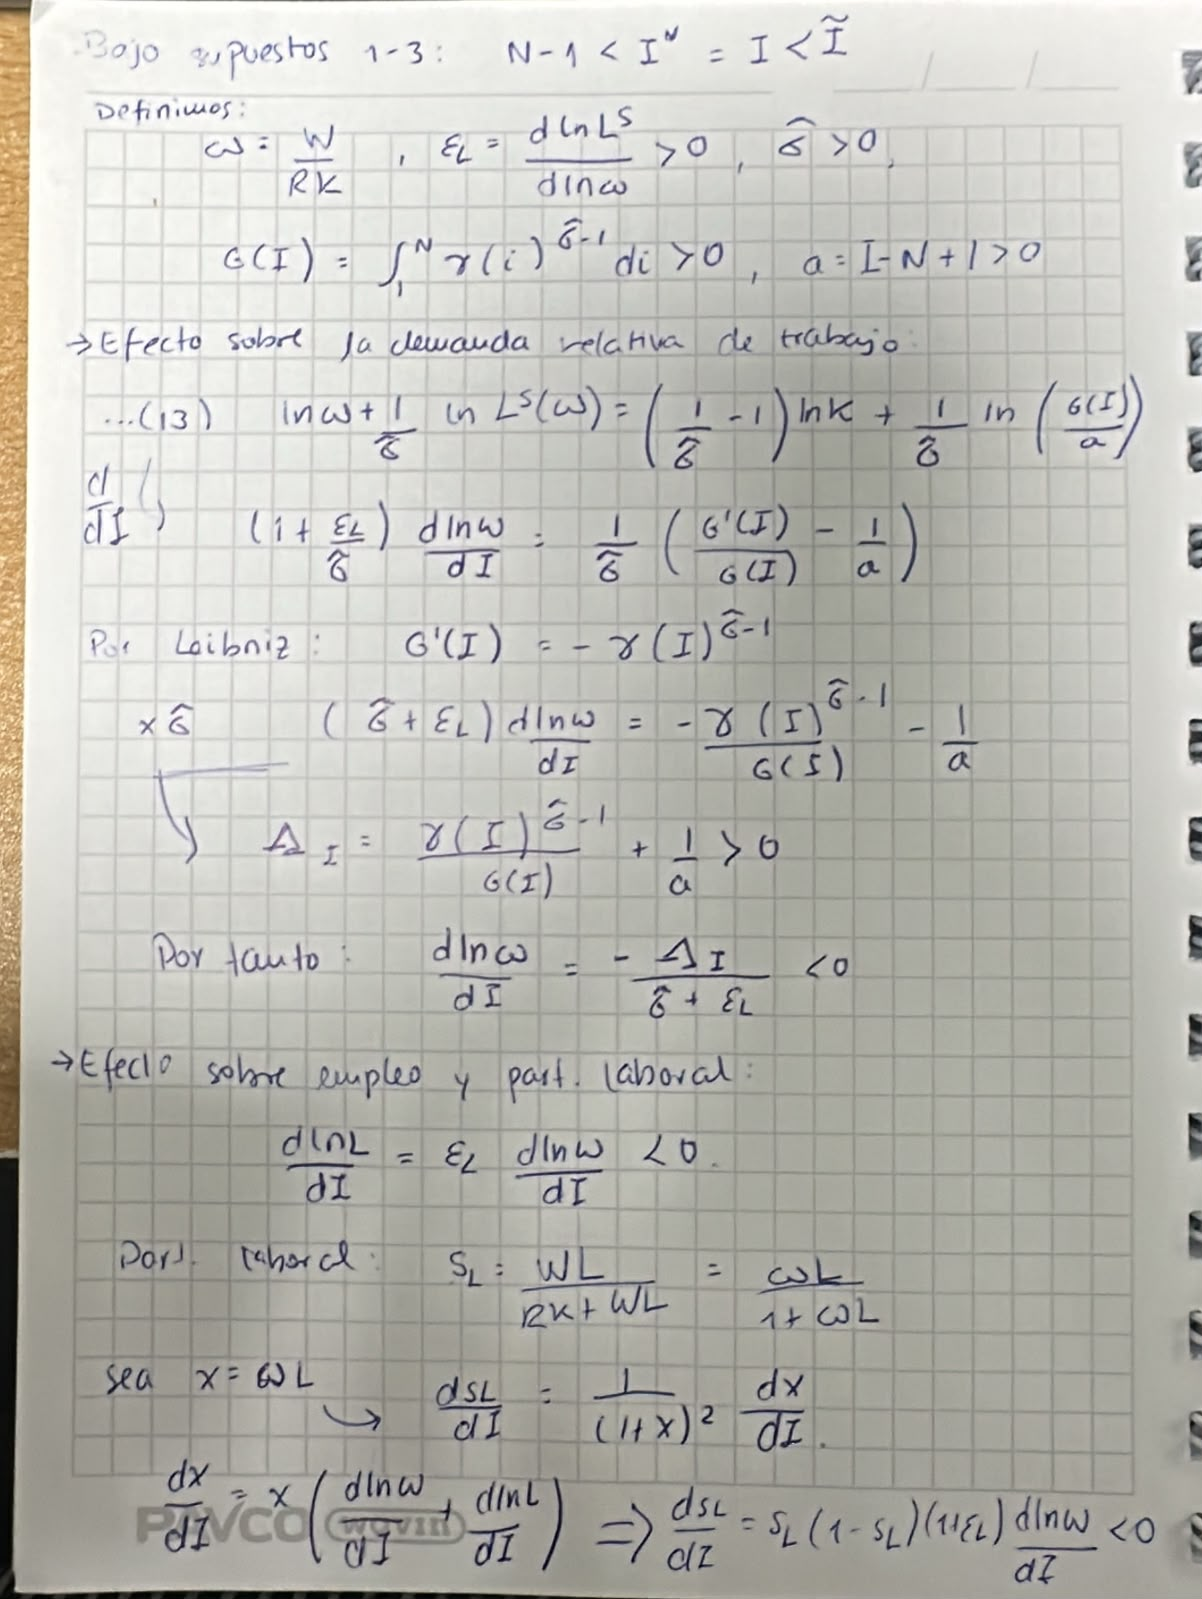
\includegraphics[height=.84\textheight]{hand/derivacion-01.jpg}
\end{frame}
\begin{frame}{Handwritten derivation: original page 2}
\centering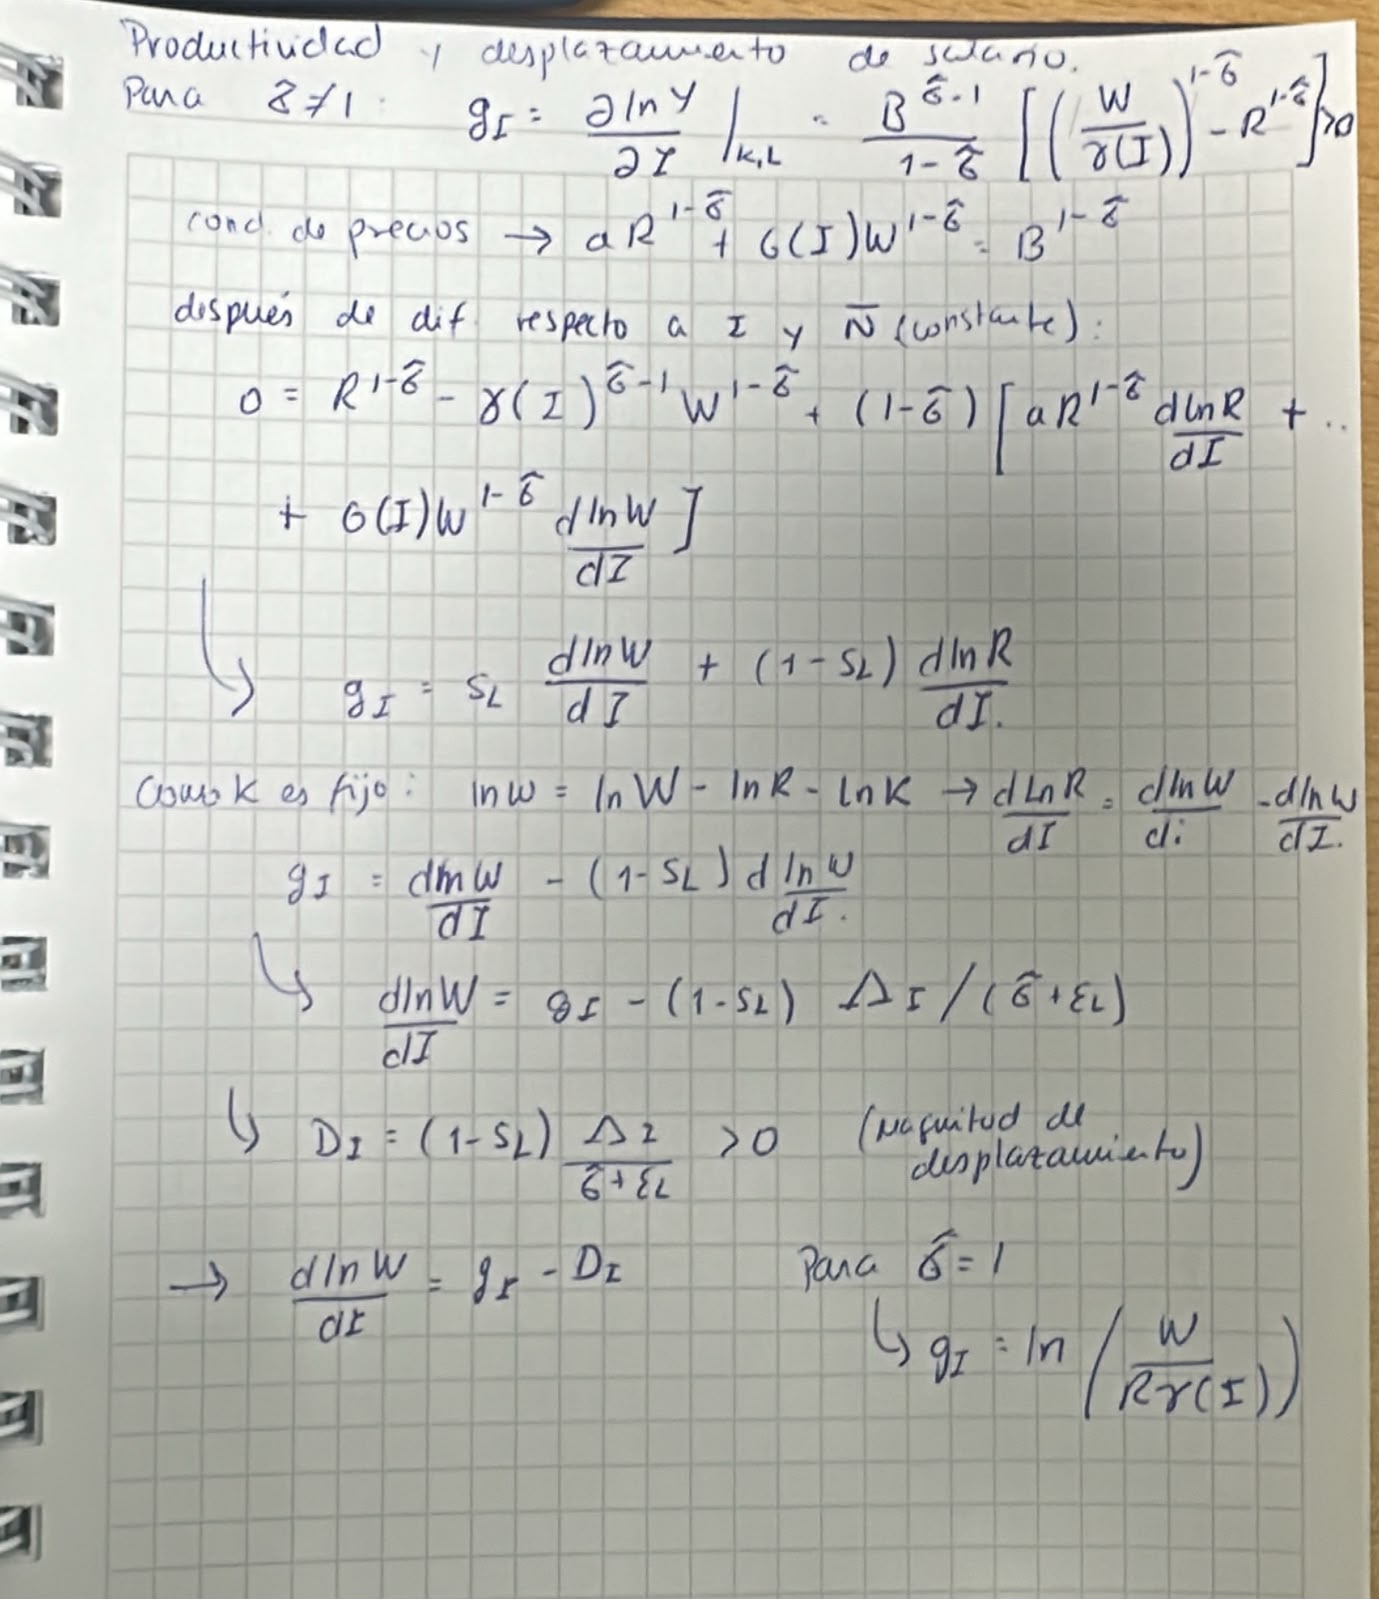
\includegraphics[height=.84\textheight]{hand/derivacion-02.jpg}
\end{frame}
\end{document}
